\section{PI Controller Pacing}
\label{sec:exp4b_results}

Experiment~4b replaces the multiplicative dual pacing of Experiment~4a with a PI controller. The $2^6$ factorial crosses auction format, aggressiveness ($a_{\text{low}}$ vs.\ $a_{\text{high}}$), market thickness ($N = 2$ vs.\ $N = 4$), budget multiplier ($m = 0.25$ vs.\ $m = 1.0$), reserve price ($r = 0.0$ vs.\ $r = 0.3$), and value dispersion ($\sigma = 0.1$ vs.\ $\sigma = 0.5$), each replicated across 50 independent seeds (3{,}200 runs total).

\begin{figure}[H]
  \centering
  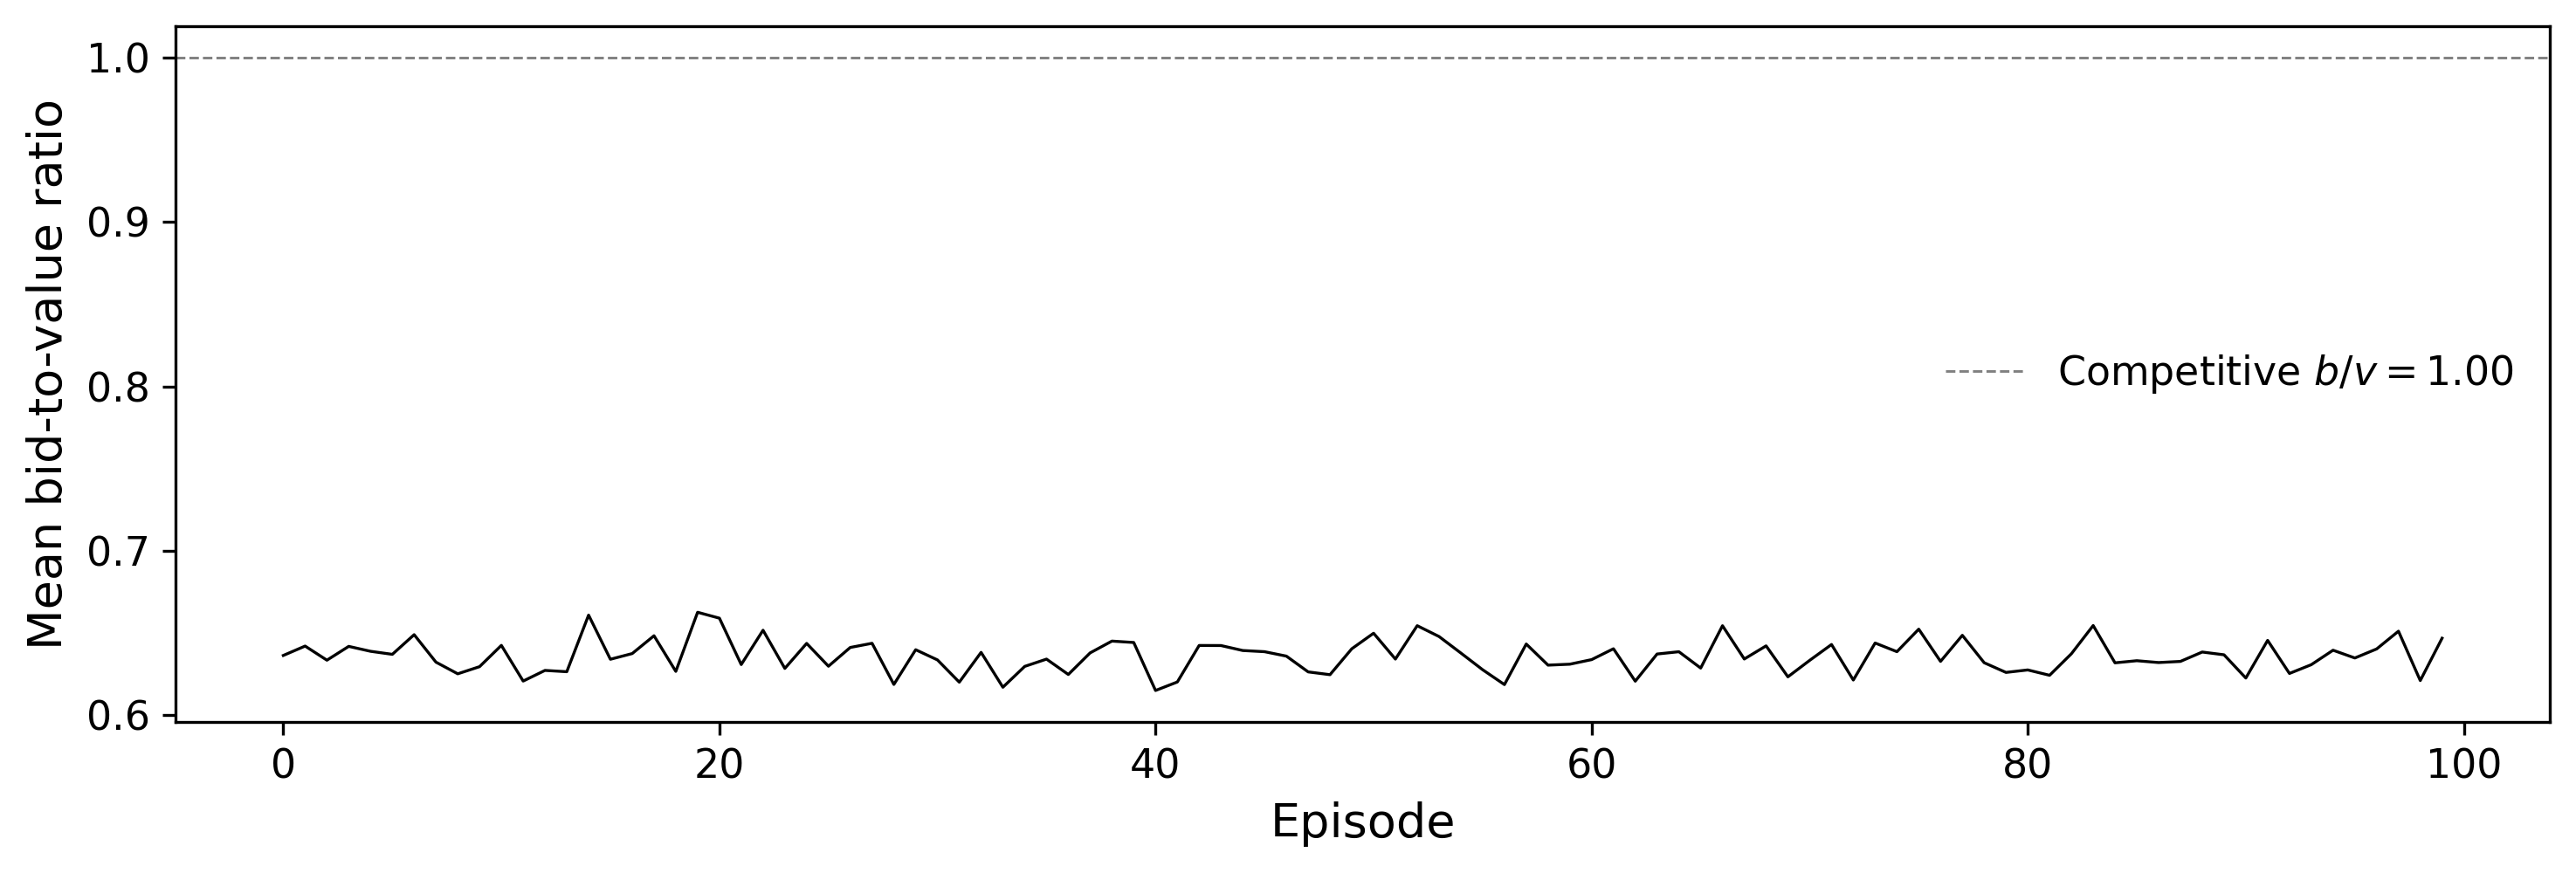
\includegraphics[width=\textwidth]{figures/e4b_trace}
  \caption{Representative learning trajectory for a single trial of Experiment~4b (first-price auction, default aggressiveness, 2~bidders, 100 episodes $\times$ 1{,}000 rounds). Mean bid-to-value ratio per episode with the competitive benchmark ($b/v = 1.0$).}
  \label{fig:e4b_trace}
\end{figure}

\subsection{Efficiency and Welfare}

The PI controller produces welfare outcomes that can be compared directly with the dual pacing results of Experiment~4a. Platform revenue and liquid welfare are computed identically, and the effective Price of Anarchy uses the same LP-based offline optimum as denominator. The budget multiplier again dominates revenue (Table~\ref{tab:exp4b_ranked_rev}), with the effect amounting to \ExpFourBRevTopPctEffect\% of the grand mean, confirming the pattern from Experiment~4a.

\input{tables/exp4b_ranked_rev}

\begin{figure}[H]
  \centering
  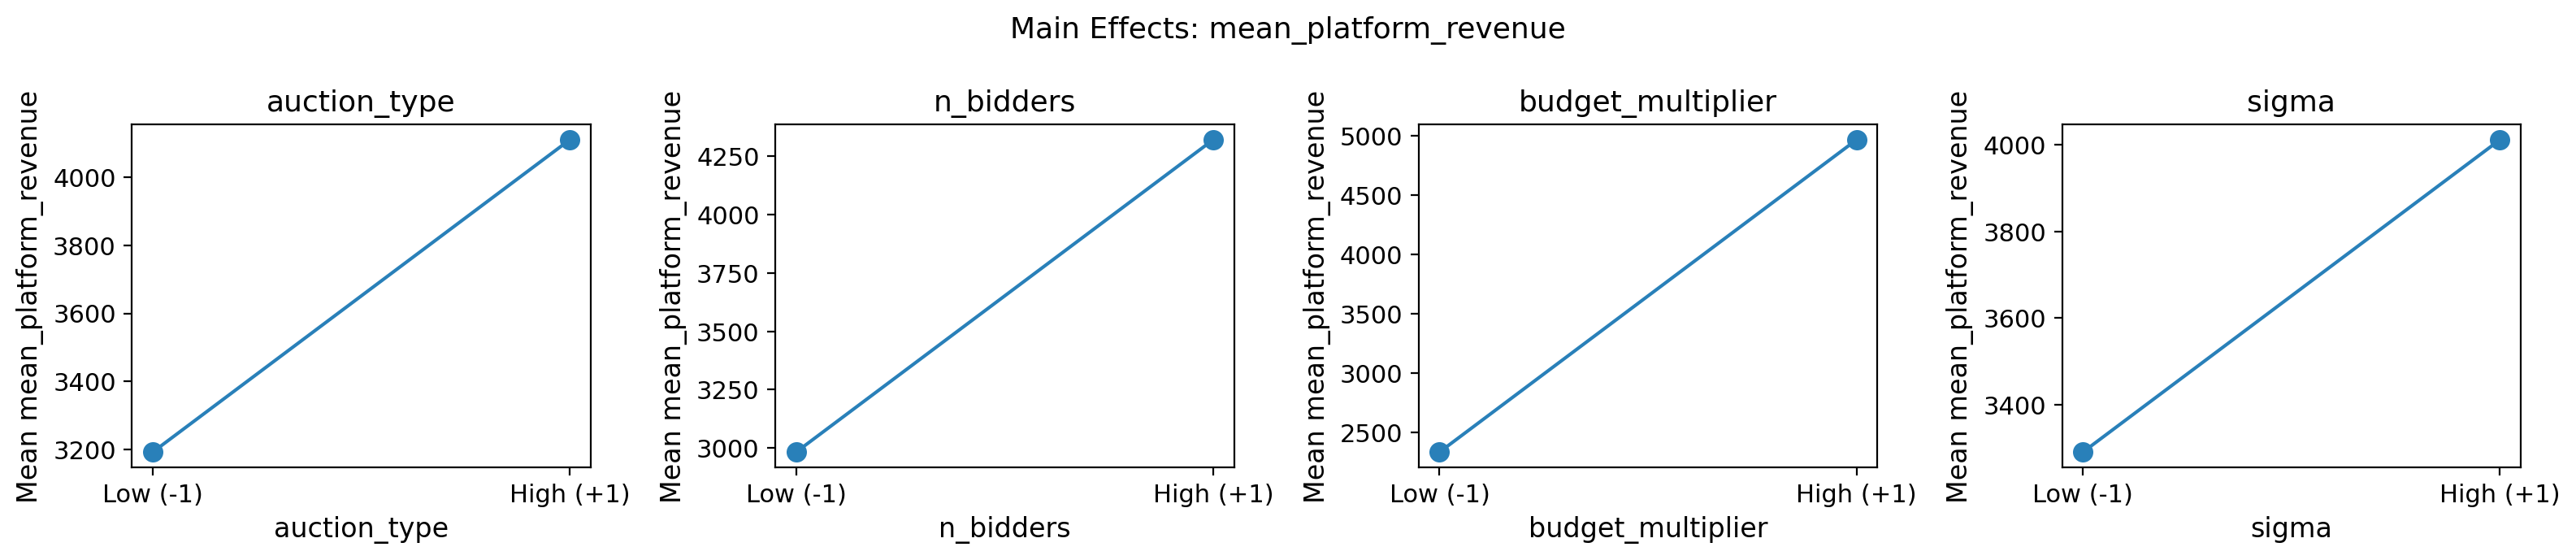
\includegraphics[width=0.7\textwidth]{figures/e4b_main_rev}
  \caption{Experiment~4b: Main effects plot for platform revenue.}
  \label{fig:e4b_main_rev}
\end{figure}

\input{tables/exp4b_ranked_poa}

\begin{figure}[H]
  \centering
  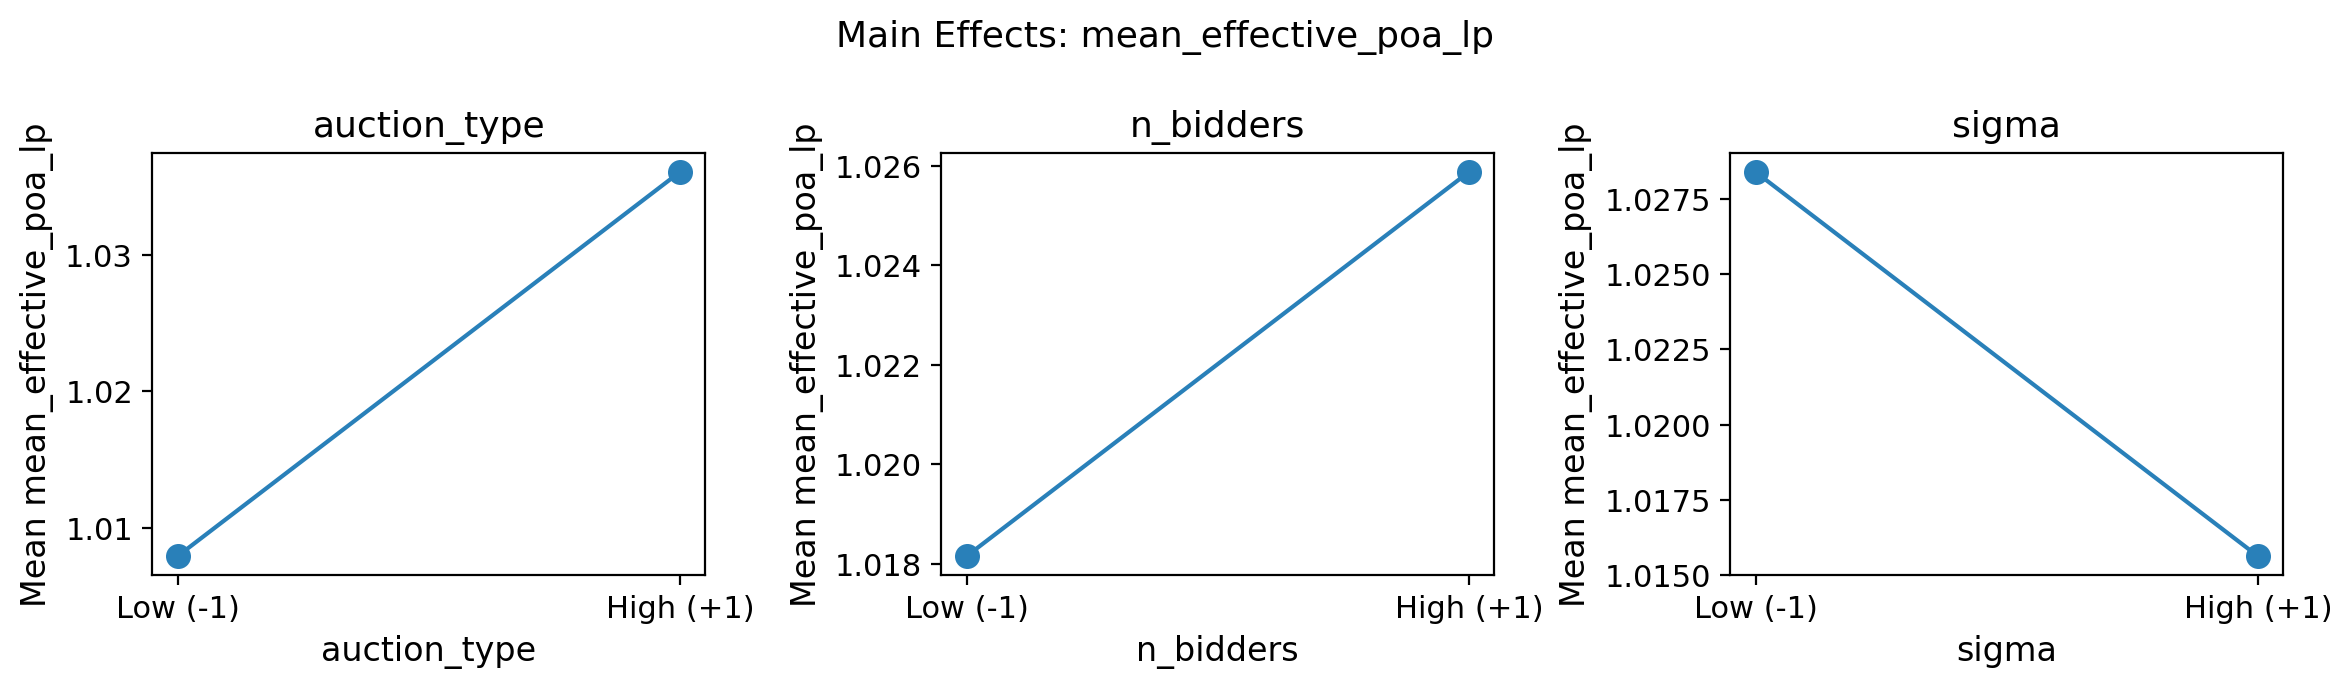
\includegraphics[width=0.7\textwidth]{figures/e4b_main_poa}
  \caption{Experiment~4b: Main effects plot for effective Price of Anarchy.}
  \label{fig:e4b_main_poa}
\end{figure}

\subsection{Revenue and Budget Dynamics}

\begin{figure}[H]
  \centering
  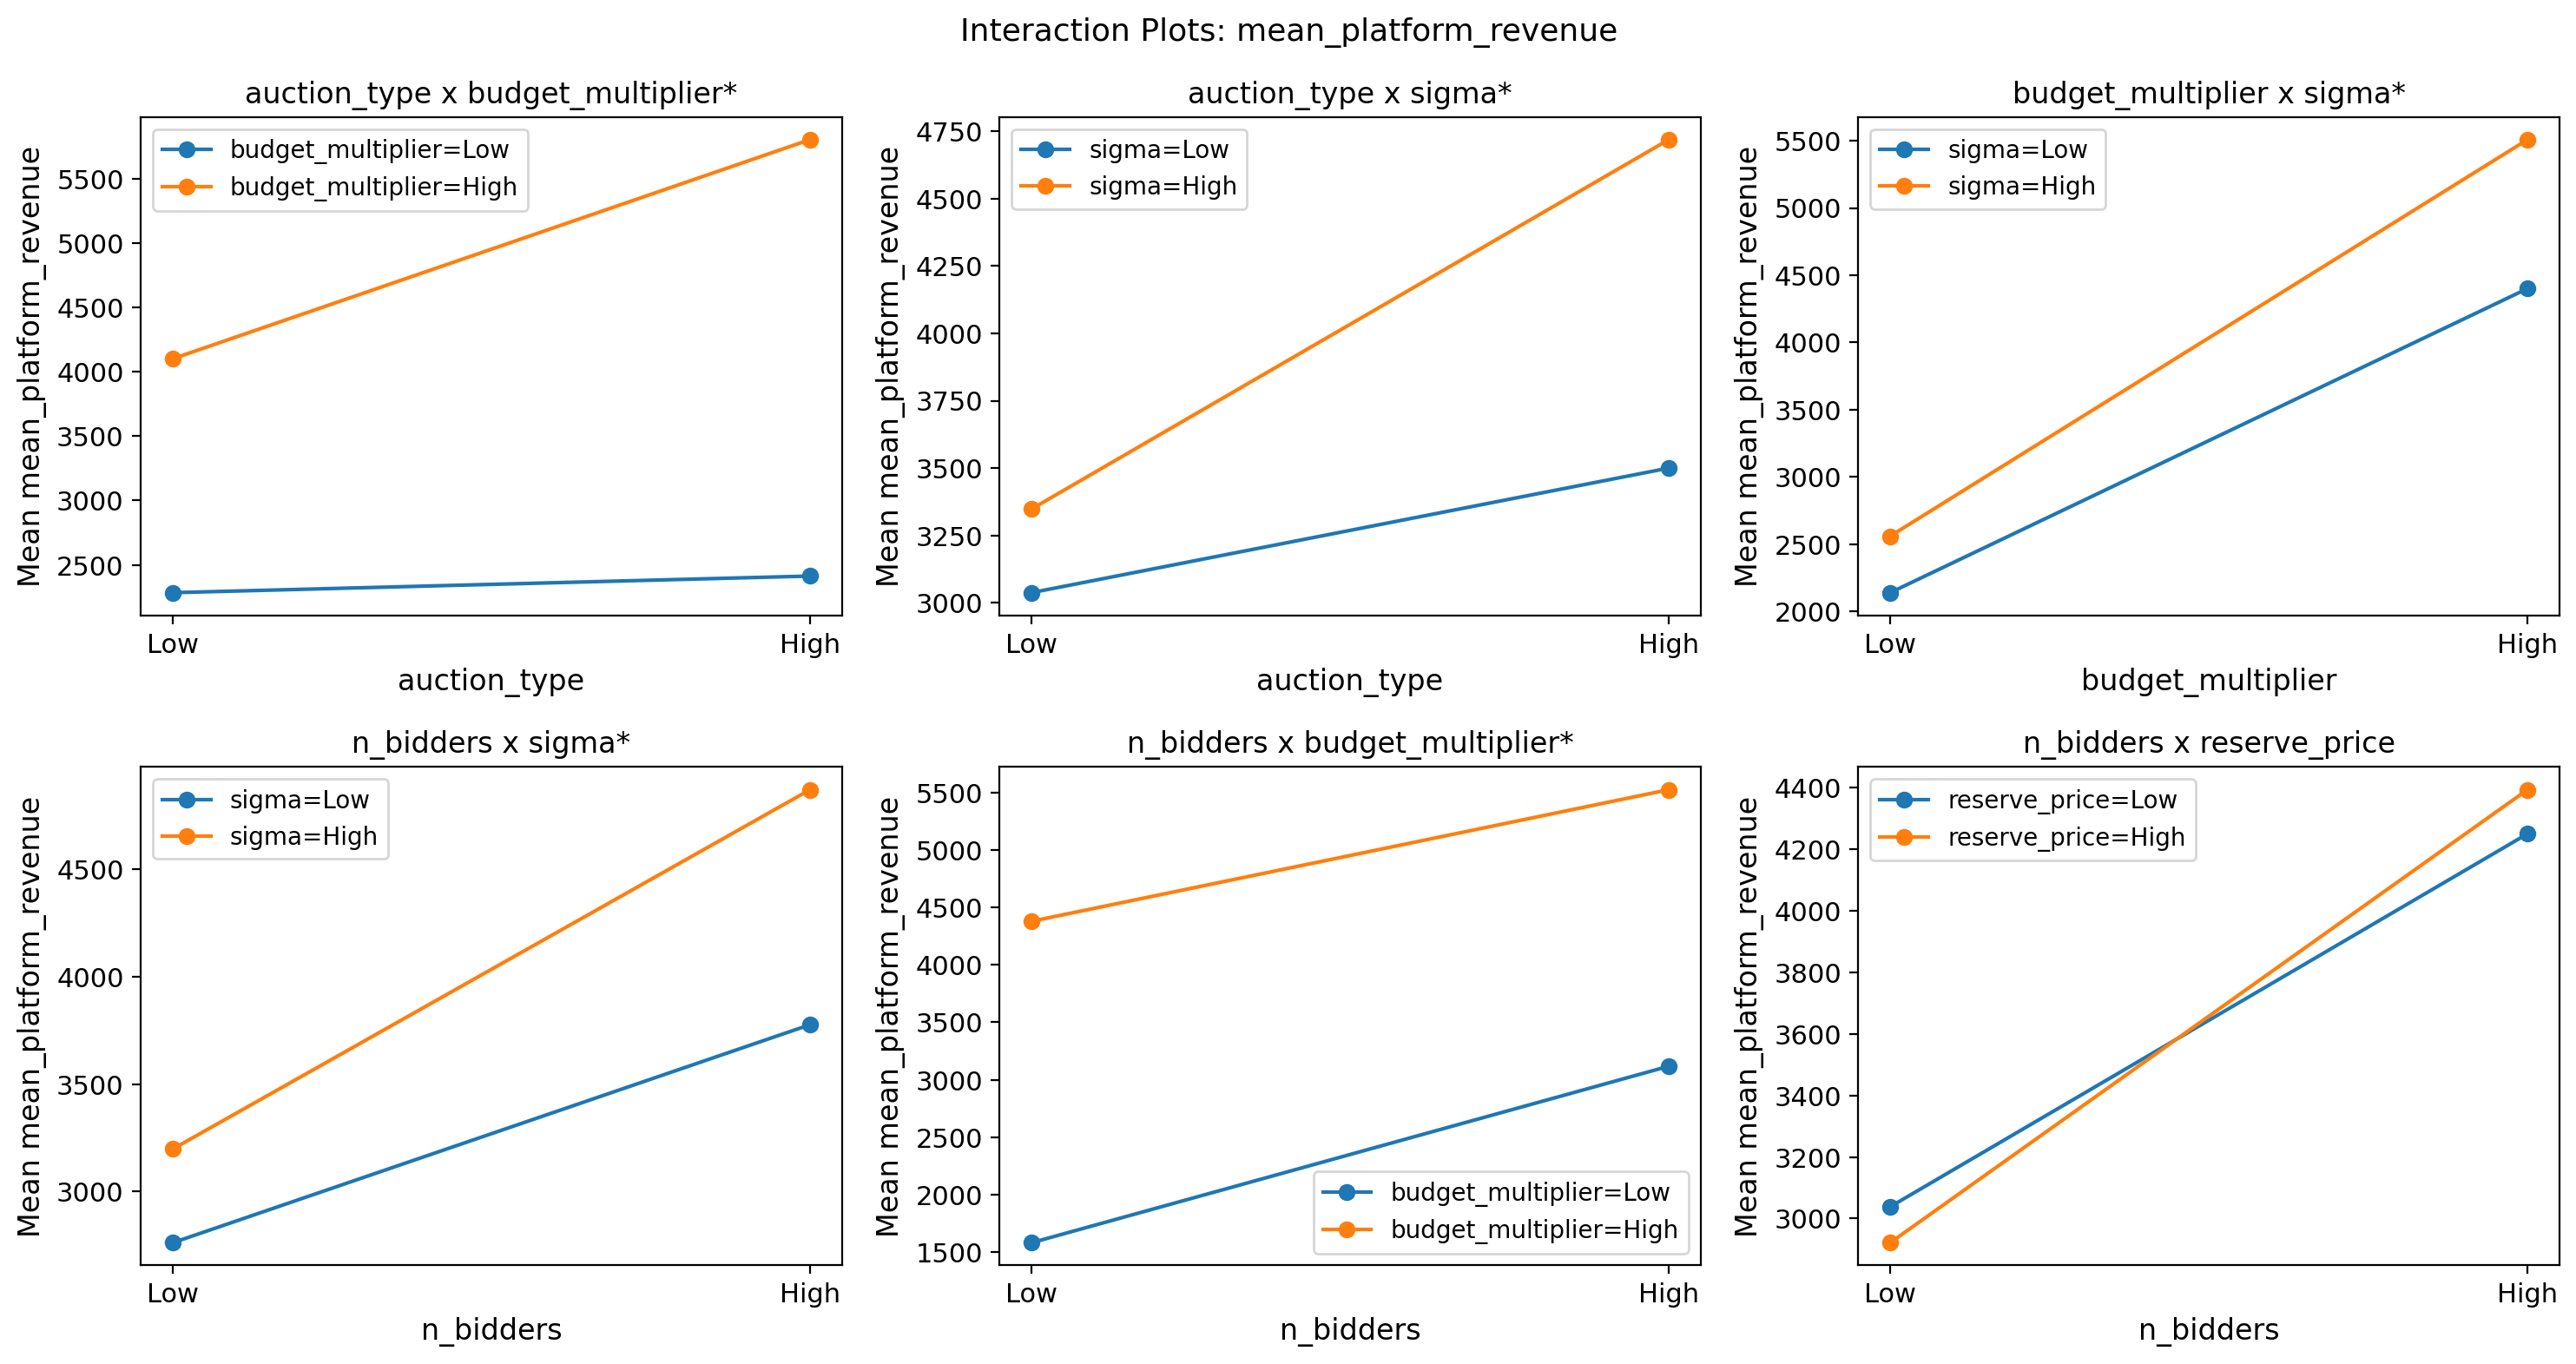
\includegraphics[width=0.7\textwidth]{figures/e4b_int_rev}
  \caption{Experiment~4b: Interaction plot for platform revenue.}
  \label{fig:e4b_int_rev}
\end{figure}

\subsection{Bidding Behaviour}

\input{tables/exp4b_ranked_vol}

\begin{figure}[H]
  \centering
  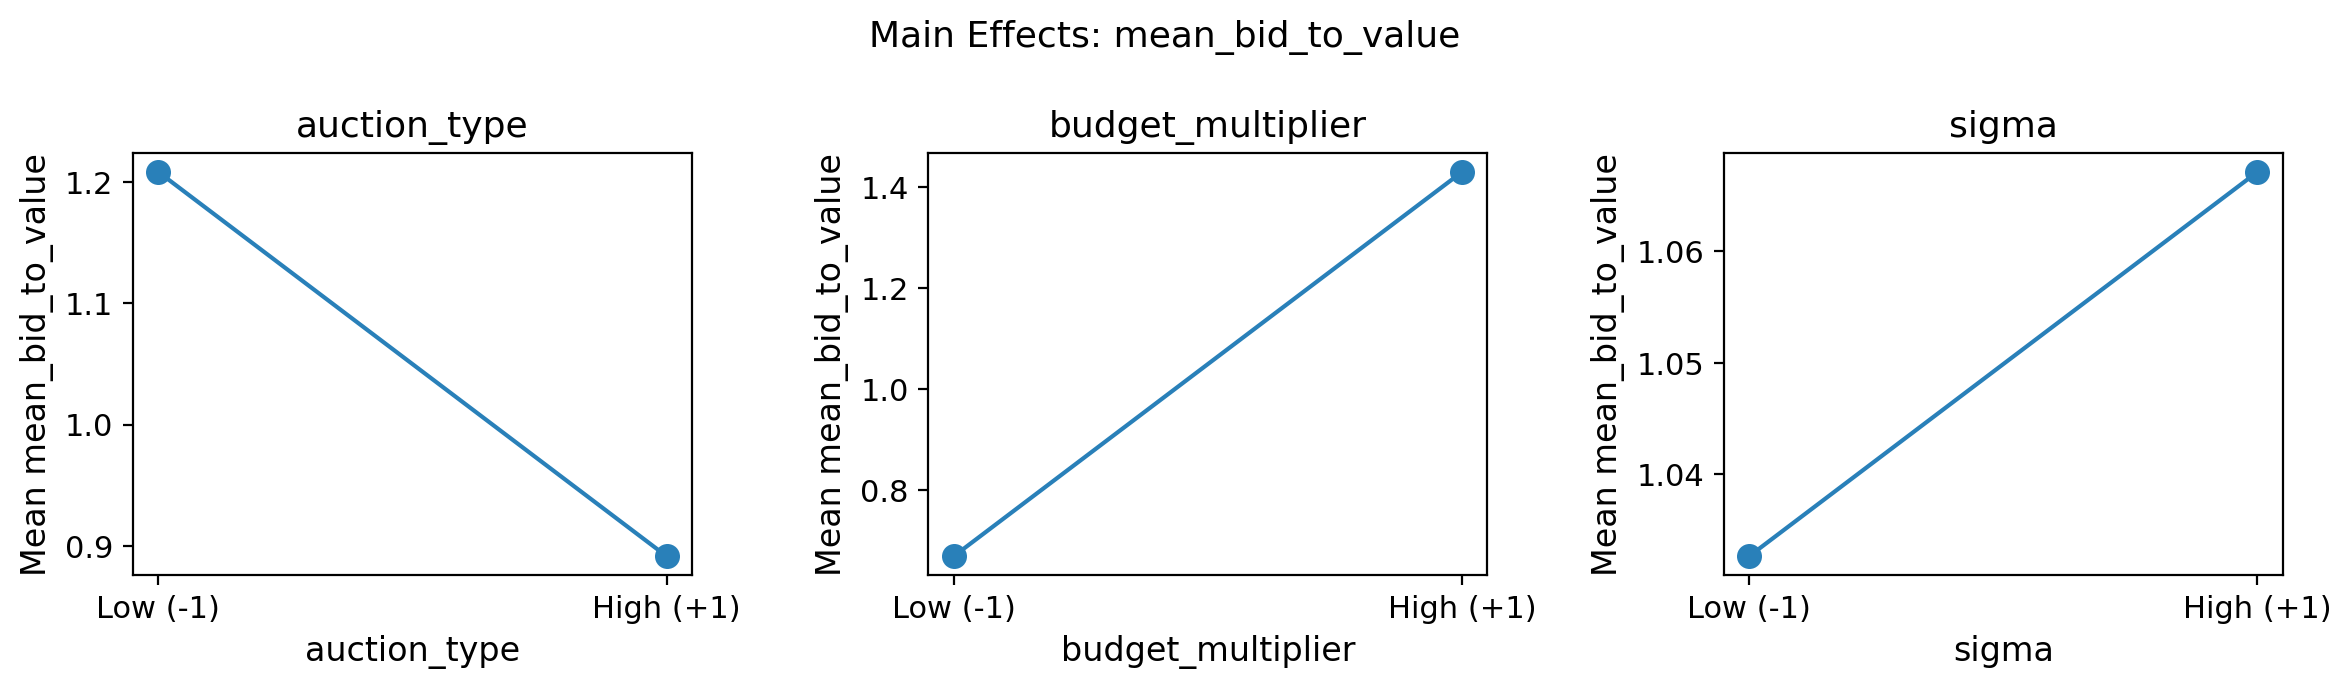
\includegraphics[width=0.7\textwidth]{figures/e4b_main_vol}
  \caption{Experiment~4b: Main effects plot for bid-to-value ratio.}
  \label{fig:e4b_main_vol}
\end{figure}

\subsection{Summary}

The comparison between multiplicative dual pacing and PI control isolates the role of the control mechanism from the budget constraint itself. As in Experiment~4a, the budget multiplier is the dominant factor ($|t| = 31.2$), with the number of bidders ranking second ($|t| = 16.1$) and auction format third ($|t| = 11.0$). All PoA values remain well within the theoretical worst-case bound of~2. The PI controller's additive updates and cumulative error tracking produce distinct bidding dynamics, but the factor hierarchy is consistent across both pacing approaches.
